\scanpage{30}
% margin note written sideways
\margin{\deleted{alors [les comp. connexes de $\Gamma\cap[s',s'']$ sont des \inserted{côtés et des} segments \unsure{$I_{\alpha}$}, des points \inserted{sommets de \deleted{\unsure{$\Gamma$}}$S$}, et les extrémités des $\unsure{I_{\alpha}}$ et] les \unsure{sg. de} $\unsure{*}$} $S(\Gamma)\cap ]s',s''[\ne\unsure{\psi|\varnothing}$, \deleted{et que, soit $t\in$} alors $\Phi:=S(\Gamma)\cap\unsure{(}T-\{s,s',s''\}\unsure{\}|\!)}\deleted{\unsure{[s',s''])}},\ne\varnothing$, et $t\in\underline{\Phi}$ réalise le maximum de la distance à la droite définie par $s',s''$, alors $]s,t[\subset\operatorname{Int}\Gamma$.}
% margin note written sideways
\margin{\uline{Corollaire} Ou bien $]s',s''[\subset\operatorname{Int}\Gamma$, ou bien $\exists\,t\in S(\Gamma)$, $t\ne\unsure{s}\unsure{\}|{}'}$, tel que $]s,t[\subset\operatorname{Int}\Gamma$.}

\figure{%
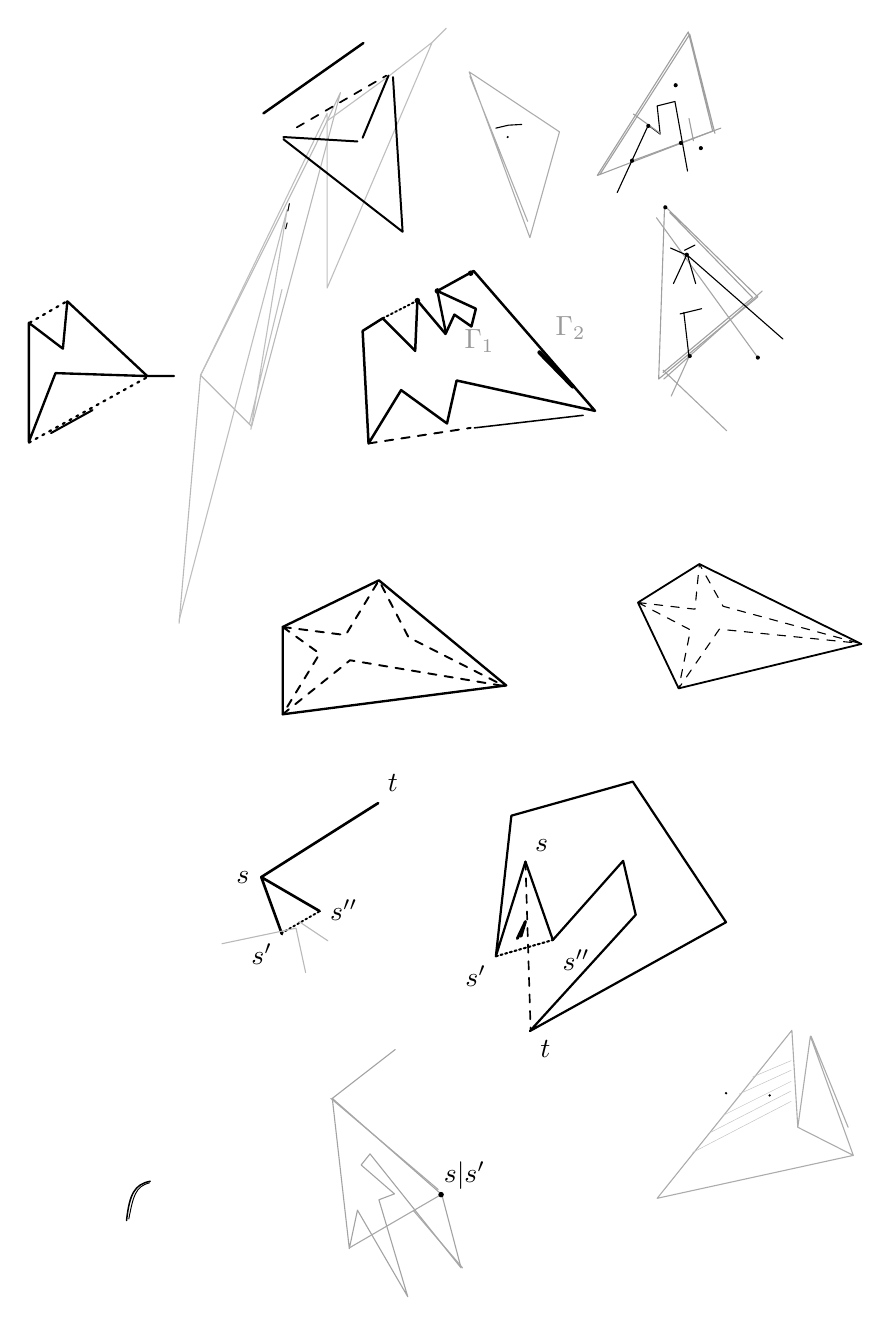
\begin{tikzpicture}[x=.0094cm,y=-.0094cm,line cap=round,line join=round]
% Pencil construction behind the dark reentrant triangle.
  \draw[gray!55] (586,906)--(615,571)--(770,261)--(804,189)--(684,640)--(615,571);
  \draw[gray!50] (586,902)--(732,347)--(683,644)
    (615,571)--(786,217)--(786,453)--(928,121)--(947,102)
    (785,228)--(869,167)--(928,121) (725,455)--(681,637);
  \draw[line width=.37pt] (735,339)--(733,349) (732,365)--(730,373);
  \draw[line width=.9pt] (700,217)--(835,122);
  \draw[line width=.72pt] (727,249)--(827,255) (834,250)--(869,166)
    (875,168)--(888,377)--(727,252);
  \draw[line width=.62pt,dashed] (745,236)--(866,166);
% Small pale triangle to the right.
  \draw[gray!65] (978,161)--(1100,242)--(1060,385)--cycle (979,167)--(1057,363);
  \draw (1014,237)--(1031,233)--(1049,232);
  \fill (1030,249) circle[radius=.43pt];
% Two upper-right pencil triangles and the strokes extended beyond their bases.
  \draw[gray!75] (1151,301)--(1274,107)--(1307,241)--cycle
    (1155,299)--(1276,110)--(1310,244);
  \draw (1178,324)--(1220,233)--(1236,245)--(1232,207)--(1256,201)--(1273,295);
  \draw[gray!75] (1200,218)--(1236,244) (1275,224)--(1281,254) (1196,282)--(1318,237);
  \foreach \p in {(1198,281),(1220,234),(1264,257),(1257,179),(1291,264)} \fill \p circle[radius=.75pt];
  \draw[gray!75] (1242,342)--(1368,465)--(1234,576)--cycle (1249,351)--(1361,466)--(1240,567);
  \draw[gray!70] (1231,358)--(1368,547) (1240,564)--(1326,646)
    (1251,599)--(1275,546) (1241,576)--(1374,457);
  \draw (1402,522)--(1272,408)--(1254,447) (1250,399)--(1273,409)--(1284,447)
    (1268,486)--(1275,546) (1263,488)--(1292,481) (1269,402)--(1283,395);
  \foreach \p in {(1272,408),(1276,545),(1243,344),(1368,547)} \fill \p circle[radius=.75pt];
% Small dark polygon beside the sideways corollary.
  \draw[line width=.85pt] (383,661)--(383,500)--(429,535)--(435,471)--(543,572)
    --(419,568)--cycle (543,572)--(579,572);
  \draw[line width=.8pt,dotted] (384,500)--(436,470) (383,662)--(542,574);
  \draw[line width=.75pt] (413,649)--(469,618);
% Large jagged polygon, including the two pale labels.
  \draw[line width=.9pt] (842,663)--(834,511)--(861,494)--(905,538)--(908,470)
    --(946,515)--(958,489)--(981,505)--(987,481)--(935,457)--(984,430)
    --(1148,619)--(961,578)--(948,636)--(886,591)--cycle;
  \draw[line width=.85pt] (935,457)--(946,511);
  \draw[densely dotted,line width=.7pt] (861,494)--(908,470);
  \draw[dashed,line width=.7pt] (842,663)--(980,642);
  \draw[line width=.55pt] (985,642)--(1132,625);
  \foreach \p in {(908,470),(935,457),(980,433)} \fill \p circle[radius=1pt];
  \draw[line width=1.55pt] (1073,540)--(1118,586);
  \node[gray!80] at (992,525) {$\Gamma_1$};
  \node[gray!80] at (1115,507) {$\Gamma_2$};
% Pair of quadrilaterals with broken interior paths.
  \draw[line width=.85pt] (726,911)--(856,848)--(1028,990)--(726,1029)--cycle;
  \draw[line width=.7pt,dashed] (726,911)--(811,922)--(856,848)--(896,925)--(1026,991)
    (726,911)--(776,947)--(726,1029)--(817,956)--(1026,991);
  \draw[line width=.65pt] (1206,878)--(1289,826)--(1508,934)--(1261,994)--cycle;
  \draw[dashed] (1206,878)--(1283,887)--(1289,826)--(1321,883)--(1505,933)
    (1206,878)--(1277,915)--(1261,994)--(1316,914)--(1505,933);
% Four-point sketch and larger labelled polygon.
  \draw[line width=.95pt] (855,1149)--(697,1249)--(725,1326) (697,1249)--(776,1295);
  \draw[densely dotted,line width=.68pt] (724,1325)--(778,1294);
  \draw[gray!55] (644,1339)--(744,1318)--(757,1378) (748,1309)--(787,1335);
  \node[left] at (694,1249) {$s$};
  \node[below left] at (725,1326) {$s'$};
  \node[right] at (777,1293) {$s''$};
  \node[above right] at (855,1147) {$t$};
  \draw[line width=.8pt] (1014,1356)--(1035,1166)--(1199,1120)--(1325,1310)
    --(1060,1457)--(1203,1300)--(1186,1227)--(1091,1334)--(1054,1228)--cycle;
  \draw[densely dotted,line width=.75pt] (1014,1356)--(1091,1334);
  \draw[dashed,line width=.6pt] (1054,1228)--(1061,1456);
  \draw[line width=1.05pt] (1043,1332)--(1054,1309)--(1048,1329);
  \node[above right] at (1054,1228) {$s$};
  \node[below left] at (1014,1356) {$s'$};
  \node[below right] at (1091,1334) {$s''$};
  \node[below right] at (1061,1456) {$t$};
% Isolated curved pen mark below the sideways corollary.
  \draw[line width=.55pt] (515,1713).. controls (519,1677) and (526,1664)..(547,1660);
  \draw[line width=.35pt] (518,1711).. controls (524,1680) and (527,1667)..(546,1662);
% Lowest pencil studies, with crossed zigzags, dots, and hatching.
  \draw[gray!72] (878,1482)--(793,1548)--(816,1751)--(827,1699)--(895,1816)
    --(856,1685)--(877,1677)--(832,1638)--(844,1623)--(967,1777)
    --(941,1678)--(793,1548);
  \draw[gray!68] (816,1750)--(940,1678) (903,1700)--(969,1777) (791,1548)--(936,1671);
  \fill (940,1678) circle[radius=1pt];
  \node[above right,inner sep=.8pt] at (940,1675) {$\unsure{s|s'}$};
  \draw[gray!65] (1232,1683)--(1414,1456)--(1422,1587)--(1439,1464)--(1497,1625)--cycle
    (1422,1587)--(1497,1625) (1440,1464)--(1490,1587);
  \foreach \x/\y/\v in {1280/1621/1552,1302/1595/1538,1321/1571/1525,1343/1542/1510,1361/1519/1497}
    \draw[gray!45,line width=.19pt] (\x,\y)--(1413,\v);
  \foreach \p in {(1325,1541),(1384,1544)} \fill \p circle[radius=.47pt];
\end{tikzpicture}}
% crop-candidate: scan 30

\uline{Lemme} Soit $\Gamma$ un \deleted{\unsure{J}}polygône \deleted{à $n\ge4$ côtés} \inserted{à $n$ côtés $(n\ge3)$}. Alors $\exists\,s\in S(\Gamma)$ \inserted{``non plat''} tel que $\forall\,D_s$ de centre $s$, \deleted{l'un des} satisfaisant la cond. b) de Déf 1, le secteur angulaire de $D$ découpé par $\Gamma$ (i.e. par $[s,s']\cup(s,s'']$ où $s',s''$ sont les $2$ sommets adjacents) qui est d'angle $>\pi$ soit \uline{extérieur} à $\Gamma$. Si $\Gamma$ est un J-polygône, et $n\ge4$, alors
\[
\begin{aligned}
&\text{(i) Si }\ \Gamma\cap\deleted{\unsure{\operatorname{Int}}}\overset{\deleted{\unsure{\circ}}}{T}=[s,s']\cup[s,s''],\quad ]s',s''[\ \deleted{\unsure{\text{est}}}\subset\operatorname{Int}\Gamma\ \text{\deleted{\unsure{et si}}}\\
&\text{(ii) Si }\ \Gamma\cap T\ne[s',s']\cup[s,s'']\quad
\deleted{\text{et }\Gamma\cap\mathring{T}=\varnothing,\ \unsure{\text{que}}\ \unsure{\Gamma\cap T}\ ]s',s''[\subset\operatorname{Int}}
\end{aligned}
\]
% archive sheet number: 29
